% Template for Cogsci submission with R Markdown

% Stuff changed from original Markdown PLOS Template
\documentclass[10pt, letterpaper]{article}

\usepackage{cogsci}
\usepackage{pslatex}
\usepackage{float}
\usepackage{caption}

% amsmath package, useful for mathematical formulas
\usepackage{amsmath}

% amssymb package, useful for mathematical symbols
\usepackage{amssymb}

% hyperref package, useful for hyperlinks
\usepackage{hyperref}

% graphicx package, useful for including eps and pdf graphics
% include graphics with the command \includegraphics
\usepackage{graphicx}

% Sweave(-like)
\usepackage{fancyvrb}
\DefineVerbatimEnvironment{Sinput}{Verbatim}{fontshape=sl}
\DefineVerbatimEnvironment{Soutput}{Verbatim}{}
\DefineVerbatimEnvironment{Scode}{Verbatim}{fontshape=sl}
\newenvironment{Schunk}{}{}
\DefineVerbatimEnvironment{Code}{Verbatim}{}
\DefineVerbatimEnvironment{CodeInput}{Verbatim}{fontshape=sl}
\DefineVerbatimEnvironment{CodeOutput}{Verbatim}{}
\newenvironment{CodeChunk}{}{}

% cite package, to clean up citations in the main text. Do not remove.
\usepackage{cite}

\usepackage{color}

% Use doublespacing - comment out for single spacing
%\usepackage{setspace}
%\doublespacing


% % Text layout
% \topmargin 0.0cm
% \oddsidemargin 0.5cm
% \evensidemargin 0.5cm
% \textwidth 16cm
% \textheight 21cm

\title{Determining the alternatives for scalar implicature}


\author{{\large \bf Benjamin Peloquin} \\ \texttt{bpeloqui@stanford.edu} \\ Department of Psychology \\ Stanford University \And {\large \bf Michael C. Frank} \\ \texttt{mcfrank@stanford.edu} \\ Department of Psychology \\ Stanford University}

\begin{document}

\maketitle

\begin{abstract}
Succesful communication regularly requires listeners to make pragmatic
inferences - enrichments beyond the literal meaning of a speaker's
utterance. For example, when interpreting a sentence such as ``Bob ate
some of the cookies,'' listeners routinely infer that Bob did not eat
all of them. A Gricean account of this phenomena assumes the presence of
alternatives (like ``all of the cookies'') with varying degrees of
informativity, but it remains an open question precisely what these
alternatives are. We use a computational model of pragmatic inference to
test out hypotheses about how well different sets of alternatives allow
us to predict scalar implicature performance across a range of different
scales. Our findings suggest that human comprehenders likely consider a
much broader set of alternatives beyond those entailed by the initial
description.

\textbf{Keywords:}
pragmatics; scalar implicature; bayesian modeling
\end{abstract}

\section{Introduction}\label{introduction}

Successful communication requires listeners to make pragmatic inferences
that go beyond the literal semantic content of speakers' utterances. For
example, listeners commonly enrich the meaning of the scalar item
``some'' to ``some but not all'' in sentences like ``Bob ate some of the
cookies'' (Grice, 1975; Horn, 1984; Levinson, 2000). These inferences,
called \emph{scalar implicatures}, have been an important test case for
understnading pragmatic inferences more generally. A Gricean account of
this phenomena assumes listeners reason about the meaning the speaker
intended by incorporating knowledge about a) alternative scalar items a
speaker could have used (such as ``all'') and b) the relative
informativity of using such alternatives (Grice, 1975). According to
this account, a listener will infer that the speaker must have intended
that Bob did not eat ``all'' the cookies because it would have been
\emph{underinformative} for the speaker to use ``some'' when ``all''
could have been used.

But what are the alternatives that should be considered in this
computation more generally? Under classic accounts of implicature,
listeners consider only those words whose meaning would entail the word
that is actually sent (Horn, 1972), and these alternatives enter into
conventionalized or semi-conventionalized scales (Levinson, 2000). For
example, because ``all'' entails ``some,'' and hence is a ``stronger''
meaning, ``all'' should be considered as an alternative to ``some'' in
implicatures. Similar scales exist for non-quantifier scales, e.g.
``love'' entails ``like'' (and hence ``I liked the movie'' implicates
that I didn't love it).

Recent empirical evidence has called into question whether entailment
scales are all that is necessary for understanding scalar implicature.
For example, Degen \& Tanenhaus (2015) demonstrated that the scalar item
``some'' was judged less appropriate when exact numbers were seen as
viable alternatives. And in a different paradigm, Tiel (2014) found
converging evidence that ``some'' was judged to be atypical for small
quantities. These data provide indirect evidence about a broader set of
alternatives: since ``some'' is logically true of sets with one or two
members, these authors argued that the presence of salient alternatives
(the words ``one'' and ``two'') reduced the felicity of ``some'' via a
pragmatic inference.

By formalizing pragmatic reasoning, computational models can help
provide more direct evidence about the role that alternatives play. The
``rational speech act'' model (RSA) is one recent framework for
understanding inferences about meaning in context (Frank \& Goodman,
2012; N. D. Goodman \& Stuhlm{ü}ller, 2013). RSA models frame language
understanding as a special case of social cognition, in which listeners
and speakers reason recursively about one another's goals. In the case
of scalar implicature, a listener makes a probabilistic inference about
what the speaker's most likely communicative goal was, given that she
picked the quantifier ``some'' rather than the stronger quantifier
``all.'' In turn, the speaker reasons about what message would best
convey her intended meaning to the listener, given that he is reasoning
in this way. This recursion is grounded in a ``literal'' listener who
reasons only according to the basic truth-functional semantics of the
language.

Franke (2014) used an RSA-style model to assess what alternatives a
speaker would need to consider in order to produce the
typicality/felicity ratings reported by Degen \& Tanenhaus (2015) and
Tiel (2014). In order to do this, Franke (2014)'s model assigned weights
to a set of alternative numerical expressions. Surprisingly, along with
weighting ``one'' highly (a conclusion that was suppored by the
empirical work),the best-fitting model assigned substantial weight to
``none'' as an alternative. This finding was especially surprising
considering the emphasis of standard theories on scalar items that stand
in entailment relationships with one another (e.g. ``one'' entails
``some'' even if it is not classically considered to be part of the
scale scale).

In our current work, we pick up where these previous studies left off,
considering the set of alternatives for implicature using the RSA model.
To gain empirical traction on this issue, however, we broaden the set of
scales we consider. Our inspiration for this move comes from work by Van
Tiel, Van Miltenburg, Zevakhina, \& Geurts (2014), who examined a
phenomenon that they dubbed ``scalar diversity,'' namely the substantial
difference in the strength of scalar implicature across a variety of
scalar pairs (e.g. ``liked/loved,'' or ``palatable/delicious.''). Making
use of some of this diversity allows us to investigate the ways that
different alternative sets give rise to implicatures of different
strengths across scales.

We begin by presenting the computational framework we use throughout the
paper. We next describe a series of experiments designed to measure both
the literal semantics of a set of scalar items and comprehenders'
pragmatic judgments for these same items. These experiments allow us to
compare the effects of different alternative sets on our ability to
model listeners' pragmatic judgements. To preview our results: we find
that standard entailment alternatives do not allow us to fit
participants' judgements, but that expanding the range of alternatives
empirically (by asking participants to generate alternative messages)
allows us to model listener judgements with high accuracy.

\section{Modeling Implicature Using
RSA}\label{modeling-implicature-using-rsa}

We begin by giving a brief presentation of the basic RSA model. This
model simulates the judgements of a pragmatic listener who wants to
infer a speaker's intended meaning \(m\) from her utterance \(u\). For
simplicity, we present a version of this model in which there is only
full recursion: that is, the pragmatic listener reasons about a
pragmatic speaker, who in turn reasons about a ``literal listener.'' We
assume throughout that this computation takes place in a signaling game
(Lewis, 1969) with a fixed set of possible meanings \(m \in M\) and a
fixed possible set of utterances \(u \in U\), with both known to both
participants. Our goal in this study is to determine what utterances
fall in \(U\).

In the standard RSA model, the pragmatic listener (denoted \(L_1\)),
makes a Bayesian inference:

\[p_{L1}(m \mid u) \propto p_{S_1} (u \mid m) p(m)\]

\noindent In other words, the probability of a particular meaning given
an utterance is proportional to the speaker's proability of using that
particular utterance to express that meaning, weighted by a prior over
meanings. This prior represents the listener's \emph{a priori}
expectations about plausible meanings, independent of the utterance.
Because our experiments take place in a context in which listeners
should have very little expectation about which meanings speakers want
to convey, for simplicity we assume a uniform prior \(p(m) \propto 1\).

The pragmatic speaker in turn considers the probability that a literal
listener would interpret her utterance correctly:

\[ p_{S_1} (u \mid m) \propto p_{L_0} (m \mid u)\]

\noindent where \(L_0\) refers to a listener who only considers the
truth-functional semantics of the utterance (that is, which meanings the
utterance can refer to).

This model of the pragmatic speaker is consistent with a speaker who
choses words to maximize the utility of an utterance in context (Frank
\& Goodman, 2012), where utility is operationalized as the informativity
of a particular utterance (surprisal) minus a cost:

\[p(u \mid m) \propto e^{-\alpha(-log(p_{L_0}(m \mid u)) - C(u))},\]

\noindent where \(C(u)\) is the cost of a particular utterance,
\(-log(p_{L_0})\) represents the \emph{surprisal} for the literal
listener (the information content of the utterance), and (\(\alpha\) is
a parameter in a standard choice rule. If \(\alpha=0\), speakers choose
randomly and as \(\alpha \rightarrow \infty\), they greedily choose the
highest probability alternative. In our simulations below, we treat
\(\alpha\) as a free parameter and fit it to the data.

To instantiate our signaling game with a tractable message set \(M\), in
our studies we adopt a food-review paradigm: we assume that speakers and
listeners are trying to communicate the number of stars in an onine
restaurant review (where \(m \in \{1, 2, 3, 4, 5\}\)). We then use
experiments to measure three components of the model. First, to measure
literal semantics \({p_{L_0} (m \mid u)}\) (we ask experiment
participants to judge whether a message is applicable to a particular
meaning (Experiment 1). Second, to generate a set of plausible
alternative messages in \(U\), we elicit alternatives directly
(Experiment 2). Lastly, to obtain human \(L_1\) pragmatic judgments, we
ask participants to interpret a speaker's utterances (Experiment 3).

\section{Experiment 1: Literal listener
task}\label{experiment-1-literal-listener-task}

\begin{CodeChunk}
\begin{figure}[t]
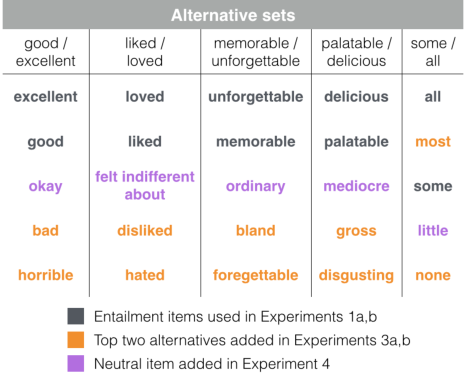
\includegraphics{figs/allScalesTable-1} \caption[Stimuli for Experiments 1, 2, and 3]{Stimuli for Experiments 1, 2, and 3}\label{fig:allScalesTable}
\end{figure}
\end{CodeChunk}

\begin{CodeChunk}
\captionsetup{width=0.8\textwidth}\begin{figure*}[t]

{\centering 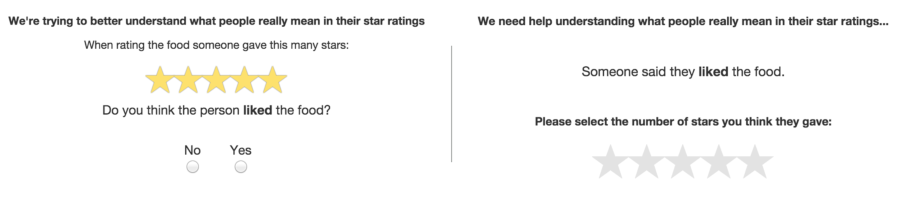
\includegraphics{figs/stimuli_exp1-1} 

}

\caption[(Left) A trial from Experiment 1 (literal listener) with the target scalar `liked]{(Left) A trial from Experiment 1 (literal listener) with the target scalar `liked.' (Right) A trial from Experiment 3 (pragmatic listener) with the target scalar `liked.'}\label{fig:stimuli_exp1}
\end{figure*}
\end{CodeChunk}

Experiment 1 was conducted to approximate literal listener semantic
distributions \(p_{L_0}(m \mid u)\) for five pairs of scalar items taken
from Tiel (2014). We include three conditions in Experiment 1,
corresponding to the sets of alternatives within a scale that
participants were presented with: two alternatives (``entailment''),
four alternatives, and five alternatives. The two-alternative entailment
condition makes a test of the hypothesis that the two members of the
classic Horn scale (Horn, 1972) are the only alternatives necessary to
predict the strength of listeners' pragmatic inference. The four- and
five-alternative conditions then add successively more alternatives to
test whether including a larger number of alternatives will increase
model
fit.\footnote{Note that alternatives in the four- and five-alternatives conditions were chosen on the basis of Experiment 2, which was run chronologically after the two-alternative condition; all literal listener experiments are grouped together for simplicity in reporting.}

\subsection{Methods}\label{methods}

\subsubsection{Participants}\label{participants}

In each condition we recruited 30 participants from Amazon Mechanical
Turk (AMT). In the two-alternative condition, two participants were
excluded because they reported having a native language other than
English for a final sample of 28 participants. In the four-alternative
condition, six participants were excluded for either failing to pass two
training trials a non-English native language, leaving a total sample of
24 participants. In the five-alternative condition, there were no data
exclusions due to training failures or native language requirements,
leaving a total sample of 30 participants.

\subsubsection{Design and procedure}\label{design-and-procedure}

Figure \ref{fig:stimuli_exp1}, left, shows the experimental setup.
Participants were presented with a target scalar item and a star rating
(1--5 stars) and asked to judge the compatibility of the scalar item and
star-rating. Compatibility was assessed through a binary ``yes/no''
response to a question of the form ``Do you think that the person
thought the food was \_\_\_\_?" where a target scalar was presented in
the blank. Each participant saw all scalar item and star rating
combinations for their particular condition (see Figure
\ref{fig:allScalesTable}), in a random oder.

The two-alternatives condition included only the scalar pairs from Tiel
(2014). The four-alternatives condition included the two scalar items
plus the top two alternatives generated for each scalar family by
participants in Experiment 2. The five-alternatives condition included
the four previous items plus one more ``neutral'' item chosen from those
alternatives generated in Experiment 2.

\subsection{Results and Discussion}\label{results-and-discussion}

\begin{CodeChunk}
\captionsetup{width=0.8\textwidth}\begin{figure*}[t]

{\centering 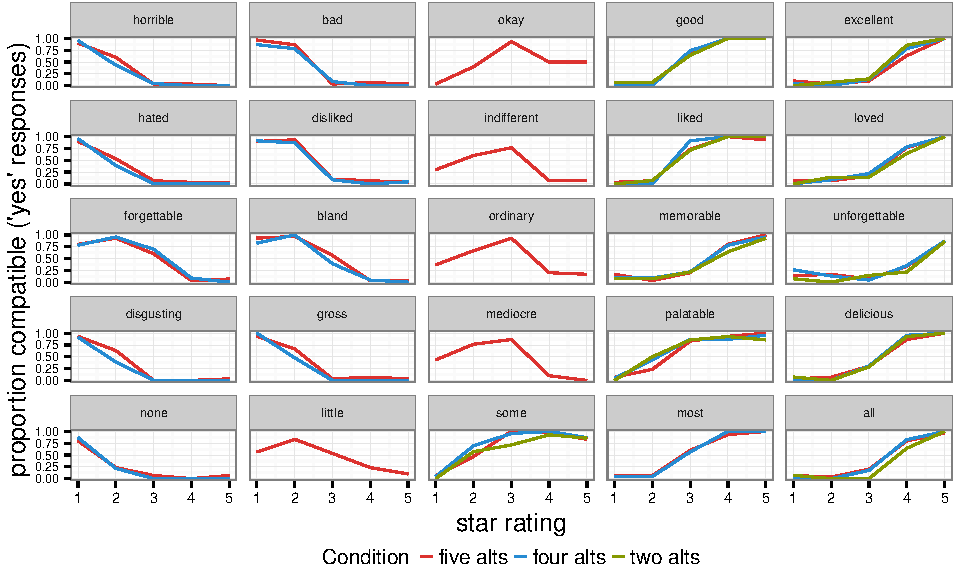
\includegraphics{figs/exp1Plots-1} 

}

\caption[Literal listener judgements from Experiments 1a, 3a, and 4]{Literal listener judgements from Experiments 1a, 3a, and 4. Proportion of participants indicating acceptability is shown on the vertical axis, with the horizontal axis showing number of stars on which the utterance was judged. Each line-type shows a different experiment, and colors indicate the different items in the scale (with the experiments including different numbers of items).  Each panel shows one scalar pair.}\label{fig:exp1Plots}
\end{figure*}
\end{CodeChunk}

Figure 2 plots literal listener \(p_{L0}(m|u)\) distributions for the
three conditions. Several trends are visible. First, in each scale, the
alternatives spanned the star scale, such that there were alternatives
that were highly compatible with both the lowest and highest numbers of
stars. Second, there was clear variability between scalar families. For
example, compatibility judgments for the top items in the ``memorable /
unforgettable'' scale were more similar than those for ``good /
excellent'' or ``liked / loved.'' Finally, there was substantial
consistency in ratings for items that were repeated across experiments,
suggesting that this paradigm elicited stable judgments from
participants.

\section{Experiment 2: Alternative
Elicitation}\label{experiment-2-alternative-elicitation}

To elicit empirical alternatives for the scales we used in Experiment 1,
we adopted a modified cloze task inspired by Experiment 2 of Tiel
(2014).

\subsection{Methods}\label{methods-1}

\subsubsection{Participants}\label{participants-1}

We recruited 30 workers on AMT. All participants were native English
speakers and naive to the purpose of the experiment.

\subsubsection{Design and procedure}\label{design-and-procedure-1}

Participants were presented a target scalar term from our original
entailment set embedded in a sentence such as, ``In a recent restaurant
review someone said they thought they the food was \_\_\_\_," with a
target scalar presented in the ``\_\_\_\_." Participants were then asked
to generate plausible alternatives by responding to the question, ``If
they'd felt differently about the food, what other words could they have
used instead of \_\_\_\_\_?'' They were prompted to generate three
unique alternatives.

\subsection{Results and Discussion}\label{results-and-discussion-1}

\begin{CodeChunk}
\captionsetup{width=0.8\textwidth}\begin{figure}[t]

{\centering 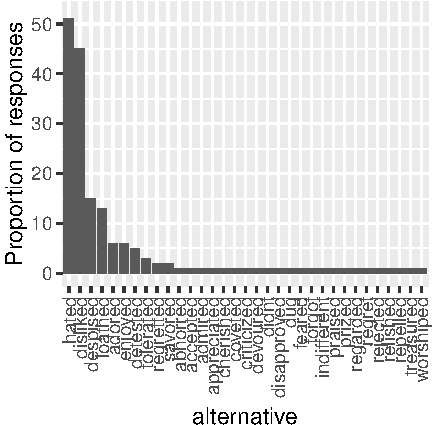
\includegraphics{figs/exp2_altsPlot_likedLoved-1} 

}

\caption[Caption goes here]{Caption goes here}\label{fig:exp2_altsPlot_likedLoved}
\end{figure}
\end{CodeChunk}

Figure \ref{fig:exp2_altsPlot} an example alternative set for the scalar
items ``liked'' and ``loved'' (combined). Alternative distributions for
the other scalar pairs (e.g.. ``good/excellent'',
``memorable/unforgettable'') were similarly long-tailed.

\section{Experiment 3: Pragmatic
Listener}\label{experiment-3-pragmatic-listener}

In Experiment 3, we asked participants to make pragmatic listener
judgements.

CONDITIONS

\subsection{Participants}\label{participants-2}

We recruited 150 participants from AMT, 50 for each condition. Data for
7 participants in the two-alternative condition were excluded after
participants either failed to pass two training trials or reported a
non-English native language, leaving a total sample of 43 participants.
In the four-alternative condition, data from five participants was
thrown out after participants either failed to pass two training trials
or were not native English speakers, leaving a total sample of 45
participants.

\subsection{Procedure}\label{procedure}

Participants were presented with a one-sentence prompt containing a
target scalar item such as ``Someone said they thought the food was
\_\_\_\_\_.'' Participants were then asked to generate a star rating
representing the rating they thought the reviewer likely gave. Each
participant was presented with all scalar items in a random order. The
experimental setup is shown in Figure \ref{fig:expt1_stimuli}, right.

\subsection{Results and Discussion}\label{results-and-discussion-2}

\section{Model Results}\label{model-results}

Using literal semantic data from Experiment 1 we conducted three
simulations with our model. Each simulation used the specific literal
semantic data to specify the scale representation available to our
model. The ``entailment'' model used only the original pair of scalar
items pulled from van Tiel (2014). These data were measured in
Experiment 1a. The ``Top two'' model extended the original set of
alternatives with the top two alternatives generated in Experiment 2.
These data were measured in Experiment 3a. The ``Full'' model included
the full set of alternatives, including a neutral valenced alternative.
These data were measured in Experiment 4.

\begin{CodeChunk}
\captionsetup{width=0.8\textwidth}\begin{figure*}[t]

{\centering 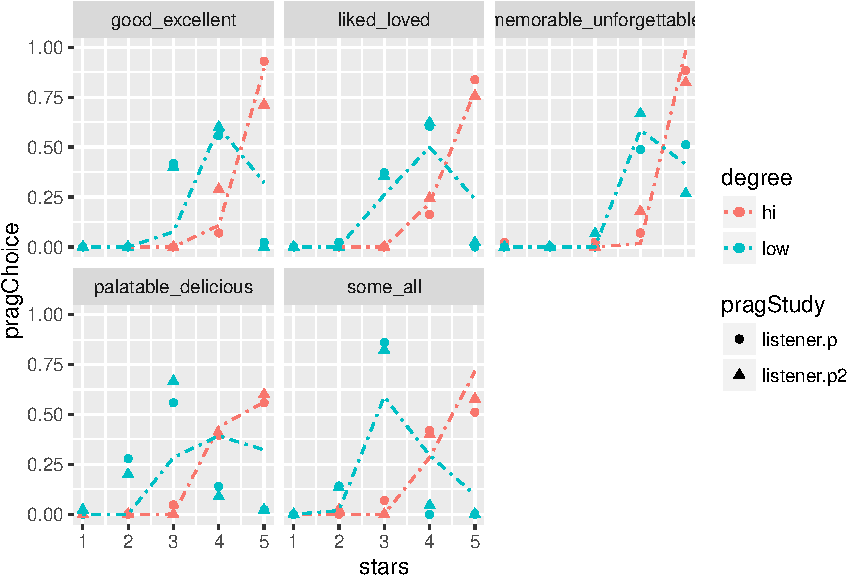
\includegraphics{figs/performancePlots-1} 

}

\caption[The left panel shows improved model fit as scale representations are enriched with more scalar items]{The left panel shows improved model fit as scale representations are enriched with more scalar items. Correlations are coputed using pragmatic judgment data from Experiments 1b and 3b. The right panel plots model predictions using full symmetric scales versus human judgments from Experiment 3b.}\label{fig:performancePlots}
\end{figure*}
\end{CodeChunk}

\section{General Discussion}\label{general-discussion}

By varying the type of scale representations available to our Bayesian
model we investigated the effects of alternatives on scalar implicature.
Model fit with human judgement was significantly improved by the
inclusion of alternatives beyond the typical ``strong'' and ``weak''
scalar items. In fact, we found that both neutral and negative valence
scalar items contribute to human-like implicature generation within our
framework.

\section{Acknowledgements}\label{acknowledgements}

Thanks to NSF BCS XYZ. Thanks to Michael Franke, Judith Degen, and Noah
Goodman.

\section{References}\label{references}

\setlength{\parindent}{-0.1in} \setlength{\leftskip}{0.125in} \noindent

Degen, J., \& Tanenhaus, M. K. (2015). Processing scalar implicature: A
constraint-based approach. \emph{Cognitive Science}, \emph{39}(4),
667--710.

Frank, M., \& Goodman, N. (2012). Predicting pragmatic reasoning in
language games. \emph{Science}, \emph{336}(6084), 998.

Franke, M. (2014). Typical use of quantifiers: A probabilistic speaker
model. In \emph{Proceedings of the 36th annual conference of the
cognitive science society} (pp. 487--492).

Goodman, N. D., \& Stuhlm{ü}ller, A. (2013). Knowledge and implicature:
Modeling language understanding as social cognition. \emph{Topics in
Cognitive Science}, \emph{5}(1), 173--184.

Grice, H. P. (1975). Logic and conversation. In P. Cole \& J. Morgan
(Eds.), \emph{Syntax and semantics} (Vol. 3). New York: Academic Press.

Horn, L. R. (1972). \emph{On the semantic properties of logical
operators.} (PhD thesis). University of California, Los Angeles.

Horn, L. R. (1984). Toward a new taxonomy for pragmatic inference:
Q-based and R-based implicature. \emph{Meaning, Form, and Use in
Context}, \emph{42}.

Levinson, S. C. (2000). \emph{Presumptive meanings: The theory of
generalized conversational implicature}. MIT Press.

Lewis, D. (1969). \emph{Convention: A philosophical study}. John Wiley
\& Sons.

Tiel, B. van. (2014). Quantity matters: Implicatures, typicality, and
truth.

Van Tiel, B., Van Miltenburg, E., Zevakhina, N., \& Geurts, B. (2014).
Scalar diversity. \emph{Journal of Semantics}, ffu017.

\end{document}
